\section{Experiments}


\subsection{Implementation}

We use the implementation of matrix factorization for inferring temporal latent spaces of a sequence of graph snapshots presented in \cite{Zhu2016}. For the classification part, we use the efficient LIBLINEAR \cite{fan2008liblinear} package and set the type of solver to L2-regularized logistic regression (primal). %that solves $min_w w^Tw/2 + C \sum log(1 + exp(-y_i w^Tx_i))$, where $w$ is the generated weight vector as the model for a given set of instance-label pairs $(x_i, y_i)$, $i$ = 1, . . . , l, $x_i \in R^n$, $y_i \in \{-1, +1\}$,  $w^Tw/2$ is the regularization term, and $C > 0$ is a penalty parameter. In the testing phase, we predict a data point $x$ as positive if $w^Tx > 0$, and negative otherwise.



%To assess the efficacy of our proposed technique, we have conduct experiments to address the following research question: \textit{Does combining latent and meta path-based topological features improve relationship prediction accuracy in DHINs?}

%We will first introduce the experiment setting, then show the results and analysis on the two types of datasets respectively.

\subsection{Experiment Setup}

\subsubsection{Dataset.} We conduct our experiments on two real-world network datasets that have different characteristics and evolution behaviour. 

\textit{Publications dataset:} The AMiner citation dataset \cite{Tang:08KDD} version 8 (2016-07-14) is extracted from DBLP, ACM, and other sources. It contains 3,272,991 papers and 8,466,859 citation relationships for 1,752,443 authors, who published in 10,436 venues, from 1936 to 2016. Each paper is associated with an abstract, authors, year, venue, and title. We confined our experiments on papers published since 1996, which includes 2,935,679 papers. Similar to \cite{sun2011ASONAM}, we also generate another dataset by considering only authors with at least 5 papers.
    
\textit{Movies dataset:} The RecSys HetRec movie dataset \cite{Cantador:RecSys2011} is an extension of MovieLens10M dataset, published by GroupLens research group that links the movies of MovieLens dataset with their corresponding web pages at IMDB and Rotten Tomatoes movie review system. It contains information of 2,113 users, 10,197 movies, 20 movie genres (avg. 2.04 genres per movie), 4,060 directors, 95,321 actors (avg. 22.78 actors per movie), 72 countries, and 855,598 ratings (avg. 404.92 ratings per user, and avg. 84.64 ratings per movie).%, and 13,222 tags (avg. 22.69 tags per user, avg. 8.12 tags per movie).

%\begin{table}[]
%\centering
%\caption{Comparison of the two networks.}
%\scriptsize
%\begin{tabular}{lllll}
%Network      & Size & Target MP & MP length & \#Training \\
%Publications &      &           &           &            \\
%Movies       &      &           &           &            \\
%             &      &           &           &           
%\end{tabular}
%\end{table}

\subsubsection{Experiment Settings.} We describe meta paths and target relationships, comparable methods, and different parameter settings.

\textit{Meta paths and target relationships}. Figure \ref{Fig:expSchema} depicts network schemas for the two datasets. Note that we consider a simplified version and ignore nodes such as topic for papers or tag for movies. Table \ref{tbl:mp} presents a number of meta paths that we consider in our experiments, where target meta path relations are \textit{co-authorship} and \textit{watching}. 
%We also limit our meta path-based measures to only path count for calculations efficiency, as the results in \cite{sun2011ASONAM} suggest that except for the case of hybrid features, using the path count measure is not considerably different than the normalized path count or the random walk. %Note that the goal of our research is not to select the best features but to show the strength of combining meta paths with temporal latent features.


\begin{figure}[t]
\centering
\subfigure[Publications Network]{
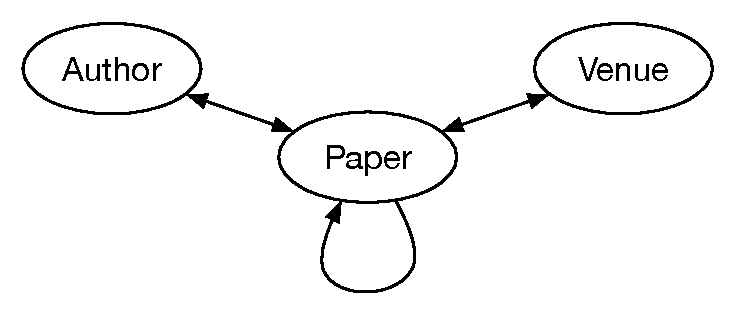
\includegraphics[trim = 0mm 0mm 0mm 0mm,width=0.45\hsize]{figs/publicationsSchema.pdf}
 \label{Fig:DBLP}
}
\subfigure[Movies Network]{
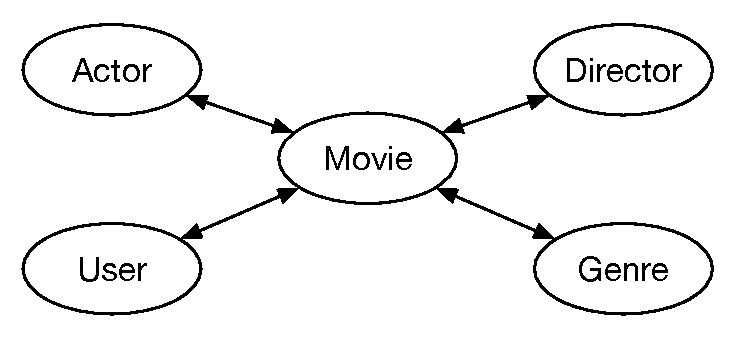
\includegraphics[trim = 0mm 0mm 0mm 0mm,width=0.45\hsize]{figs/moviesSchema.pdf}
 \label{Fig:IMDB}
}
\caption{The simplified network schema used for our experiments.} \label{Fig:expSchema}
\end{figure}


\begin{table}[t]
\centering
\caption{Meta paths for publications dataset with $V$=\{Author, Paper, Venue\} and movies dataset with $V$=\{User, Movie, Actor, Director, Genre\}.}
\label{table_publications}\scriptsize\label{tbl:mp}
\begin{tabular}{|l|c|l|} \hline
\textbf{Network} & \textbf{Meta path} & \textbf{Meaning} \\ \hline

\multirow{4}{*}{Publications} & \textit{A--P--A} & [\textit{The target relation}] Authors are coauthors \\ \cline{2-3}
& \textit{A--P--V--P--A} & Authors publish in the same venue \\ \cline{2-3}
& \textit{A--P--A--P--A} & Authors have the same co-author \\ \cline{2-3}
& \textit{A--P--P--P--A} & Authors cite the same papers \\ \hline

\multirow{5}{*}{Movies} & \textit{U--M} & [\textit{The target relation}] A user watches a movie \\ \cline{2-3}
& \textit{U--M--A--M} & A user watches a movie with the same actor \\ \cline{2-3}
& \textit{U--M--D--M} & A user watches a movie with the same director \\ \cline{2-3}
& \textit{U--M--G--M} & A user watches a movie of the same genre \\ \cline{2-3}
& \textit{U--M--U--M} & A user watches a movie that another user  \\ \hline

\end{tabular}
\end{table}

%For the publications network we consider meta paths \textit{A-P-V-P-A}, \textit{A-P-A-P-A}, and \textit{A-P-P-P-A}, as the study in \cite{sun2011ASONAM} shows that shared co-authors, shared venues, and co-cited papers for two authors significantly contribute to their future collaborations. There are two major differences between target relation types in our datasets. First, unlike a new co-authorship relation that happens at a particular time, users can watch/rate a movie once it is released. In other words each paper is published once and a new co-authorship is made at that time whereas users create new watching relations to an existing movie. Second, the target relation for the publications dataset, i.e., \textit{A-P-A}, has the same node type at both ends, while the target meta path for the movie dataset, i.e., \textit{U-M}, considers two different node types. Note that $G^\mathcal{P}_i$s in Equation 1 are square adjacency matrices. For the case of having target relations with two types of nodes at ends, we consider 0 value for the relationships of the same type in case no such relation actually exists in the network.

%to show the effectiveness of our proposed methods in predicting such relationships. 


%conducted Wald test in a case study and found that the $p$-value for the feature associated with each meta path and their significance level. From the results, we can see that the 

% Movies
%Out of 12310, 10109 movies were rated movies



\textit{Comparable methods.} We perform comparative analysis of our work, denoted as \textit{MetaDynaMix}, with four techniques: (1) The original \textit{PathPredict} that considers only 3 intervals \cite{sun2011ASONAM}, (2) PathPredict applied on different time intervals, denoted as \textit{PathPredict2}, (3) homogenized link prediction (Section \ref{def:HLP}), denoted as \textit{HLP}, and (4) logistic regression on HLP latent features, denoted as \textit{LRHLP}. %The state-of-the-art methods which we compare against are \textit{PathPredict} \cite{sun2011ASONAM}, and matrix factorization for temporal prediction \cite{Zhu2016} (denoted as \textit{BCGD}). 
Sun et al. \cite{sun2011ASONAM} showed that \textit{PathPredict} outperforms traditional link prediction approaches that use topological features defined in homogeneous networks such as common neighbors or Katz$\beta$, and thus we do not include these techniques in our experiments.


%\begin{itemize}
%    \item  Heterogeneous non-temporal (PathCount, PathSim, NormalPathCount, RandomWalk, SymmetricRandomWalk)
%    \item  Homogeneous non-temporal (Katz, Jaccard)
%    \item  Homogeneous temporal (BCGD)
%\end{itemize}


\textit{Parameters.} We set the number of snapshots $t$=3, 5, and 7 to evaluate the effect of dynamic analysis of different time intervals. Note that $t$=3 refers to the default case for many link prediction algorithms that learn based on one interval and test based on another interval. More specifically in the training phase features are extracted based on T1 and labels are determined based on T2, and for the testing phase features are calculated based on T2 and labels are checked across T3. We also set the number of latent features $k$ to 10, 15, and 20.

\subsubsection{Evaluation Metrics.} 

To asses link prediction accuracy, we use Area Under Curves (both Receiver Operating Characteristic (ROC) and Precision-Recall (PR) curves), termed as AUCROC and AUCPR \cite{davis2006relationship}. We also present the prediction accuracy for 5-fold cross validation. Furthermore we perform the non-parametric McNemar's test \cite{mcnemar1947note} to assess the statistical significance of the difference between the classifiers accuracy of different techniques.

\subsection{Results and Findings}

%DBLP
    179,607 authors had no co-author in 1996-2016. 
    78,635 authors had no co-author (about 4\%). 
    ------------
    100,972 (those who published in 1930-1996)?
    
    1,752,443 (total) - 100,972 = 1,651,471 (those who published in 1996-2016)?
    
    1,544,408 authors had no co-author in 1930-1996
    78,635 authors had no co-author (about 4\%). 
    ------------
    1,465,773 (those who published in 1996-2016)?

    1,752,443 (total) -1,465,773 = 300,000 (those who published in between)?
    
%    1,752,443 author_papervenuelist_map
%    2,811,533 paper_authorslist_map
%    10,163 venue_paperauthorslist_map
    
78,635 authors had no co-author (about 4\%)

Adding more features to our Logistic Regression model will increase the training accuracy because model has to consider more data to fit the logistic regression. But testing accuracy increases if feature is found to be significant

The null hypothesis of the McNemar's states that the same population proportion of links will be correctly classified by the two methods. However the test result gives a $p$-value $<$ 0.0001 and hence we reject the null hypothesis of equal classifier performance.

\amin{One reason that \textit{A--P--V--P--A} is better with intervals is that one may publish in ECIR but there are so many publishing there....}
